\documentclass{beamer}
\usepackage[utf8]{inputenc}
\usepackage{graphicx}
\graphicspath{ {./images/} }

\title{Vývoj samoříditelné platformy}
\author{Filip Peterek}
\institute{Vysoká škola Báňská - Technická univerzita Ostrava}
\date{Květen 2021}

\AtBeginSection[]{
    \begin{frame}
        \frametitle{Obsah}
        \tableofcontents[currentsection]
    \end{frame}
}

\begin{document}

\frame{\titlepage}

\section{Cíl práce}
\begin{frame}
    \frametitle{Cíl práce}

    \begin{itemize}
        \item Prozkoumat možnosti autonomního řízení vozidla
        \item Implementovat autonomní řízení v kampusu VŠB-TUO
        \item Implementovat komunikaci s vozidlem pomocí rozhraní CAN
        \item Implementovat simulátor vozidla sloužící k testování SW
    \end{itemize}

\end{frame}

\section{Výsledek práce}
\begin{frame}
    \frametitle{Výsledek práce}
    
    \begin{itemize}
        \item Následování grafických kódů
        \item Nefunkční řízení pomocí GPS
        \item Rozpracované řízení využívající vstupů z kamer, LiDARu i GPS
        \item Webová aplikace sloužící k ovládání vozidla
        \item Python skript sloužící ke stahování a exportu mapových podkladů
        \item Simulátor vozidla
        \item Komunikace s vozidlem za využití rozhraní CAN
        \item Android aplikace logující GPS souřadnice
    \end{itemize}
\end{frame}

\section{Architektura projektu}

\begin{frame}
    \frametitle{Architektura projektu}
    \begin{center}
        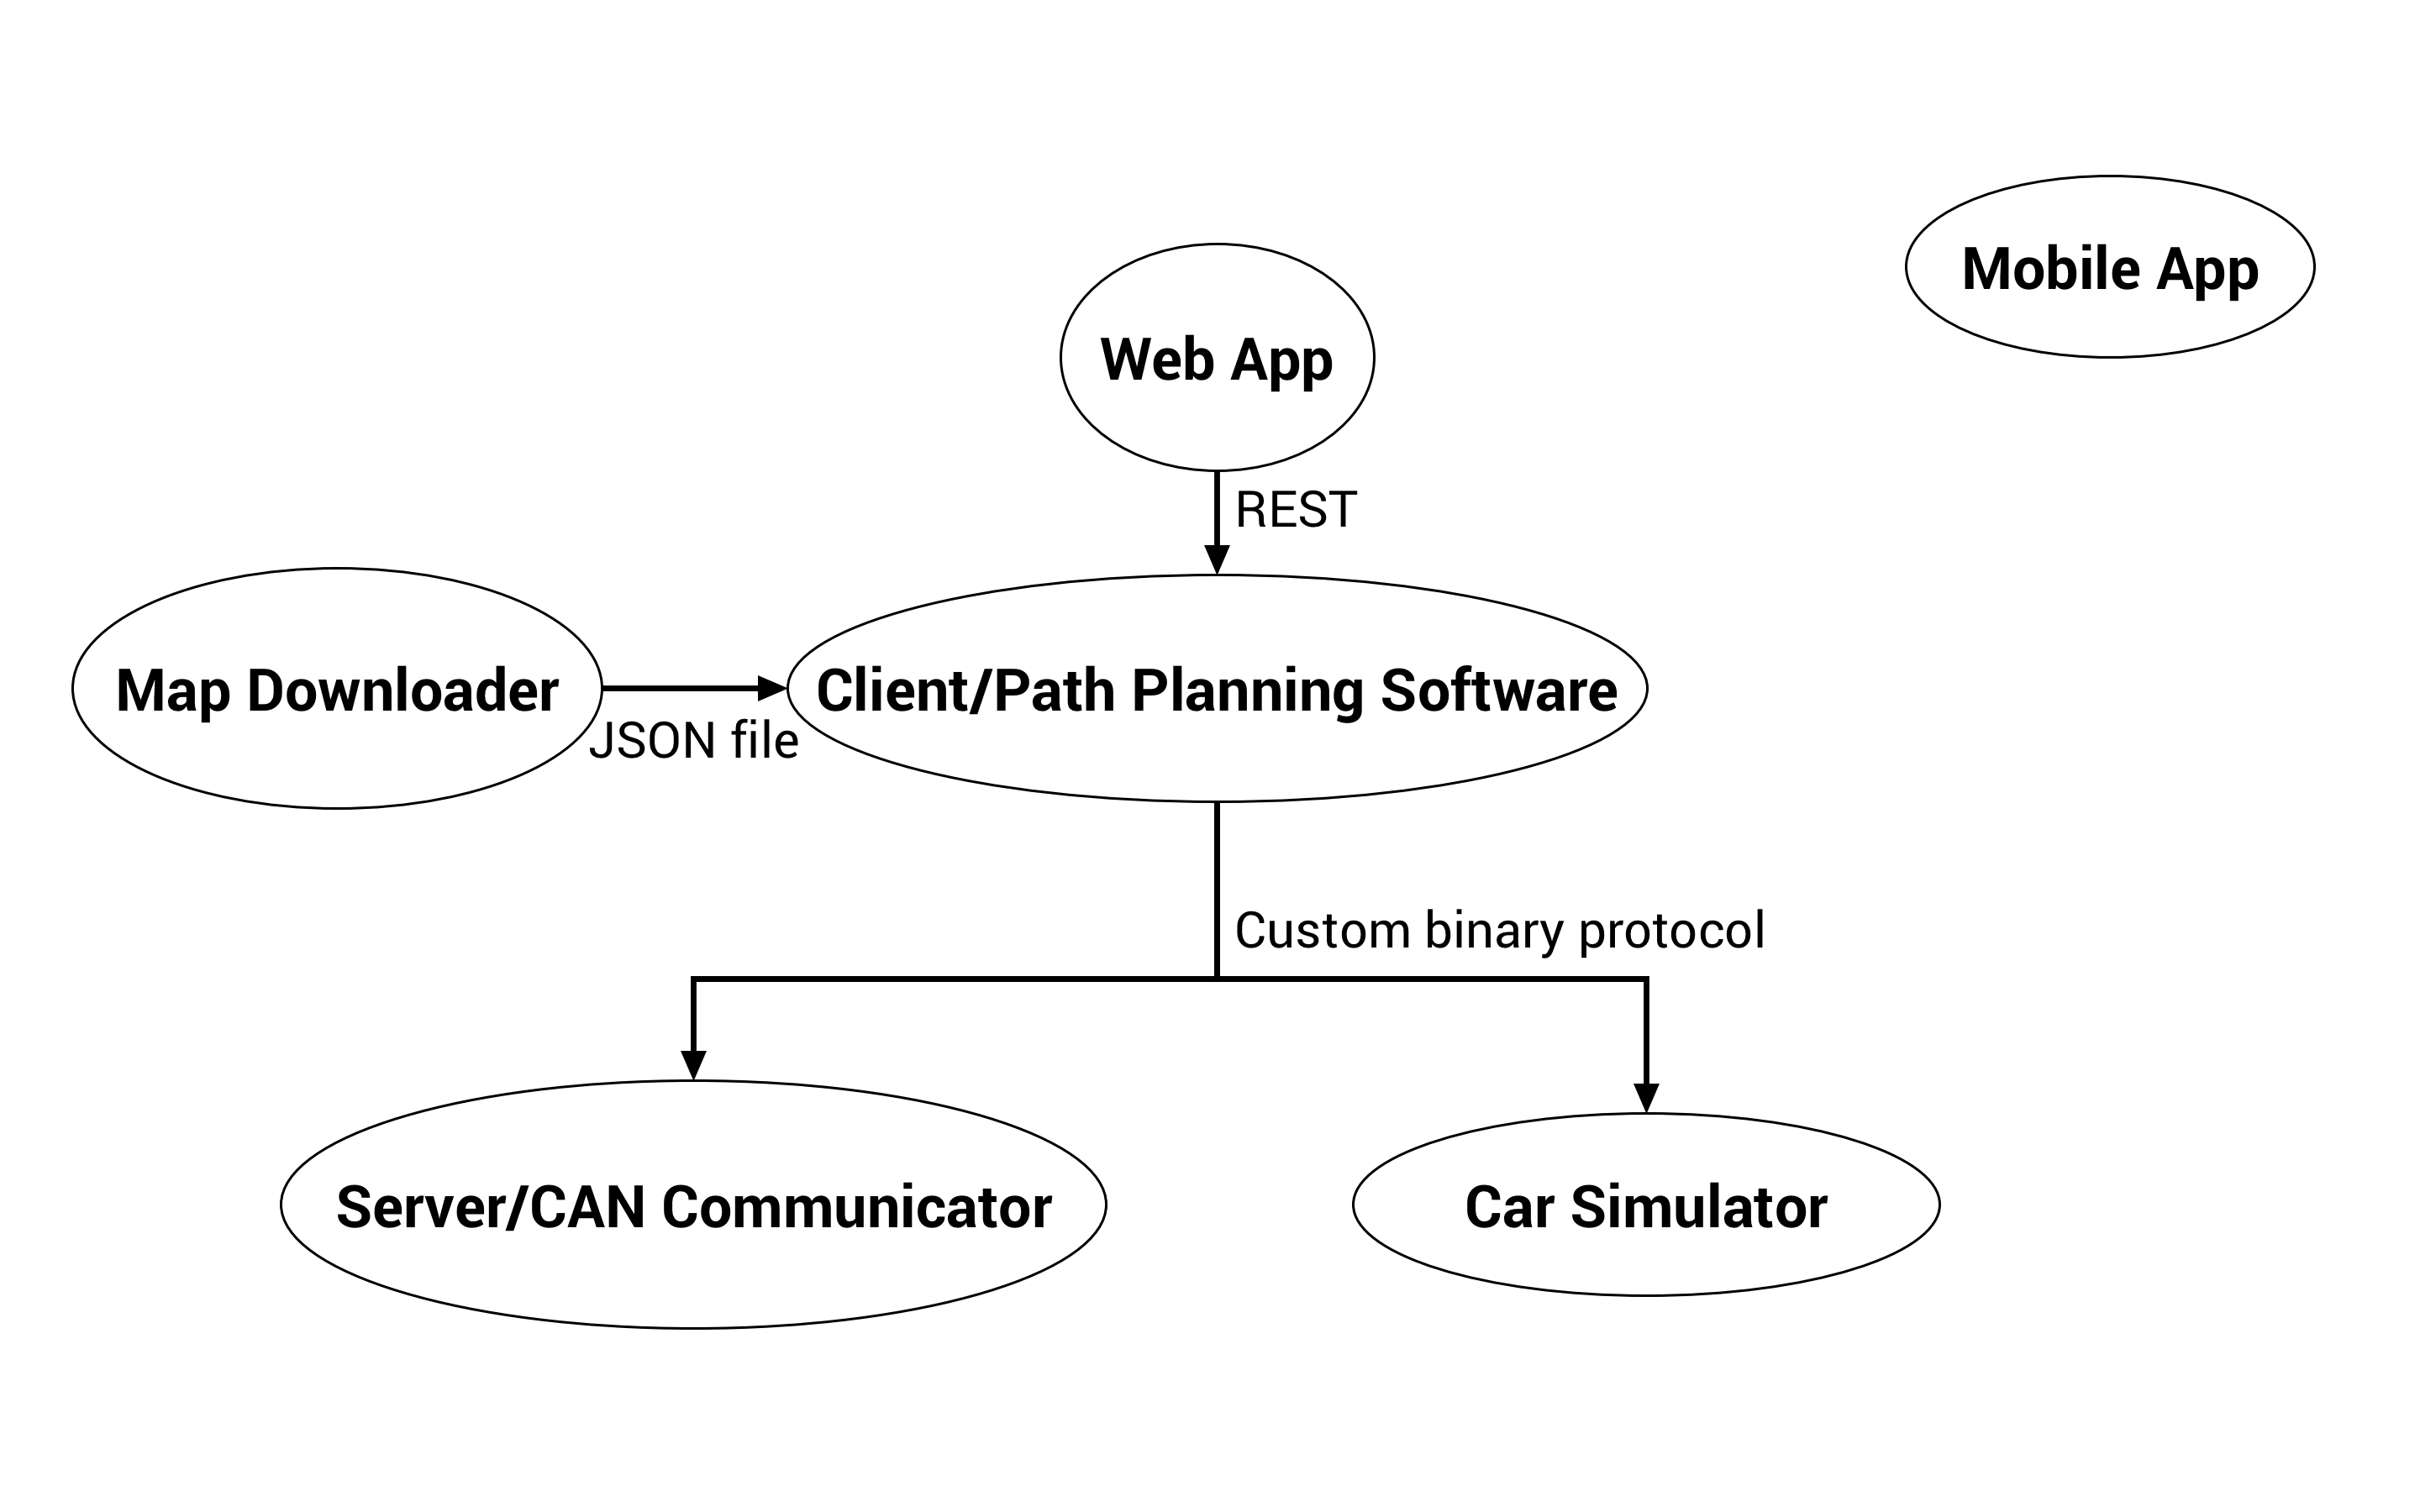
\includegraphics[width=0.9\columnwidth]{car-schema}
    \end{center}
\end{frame}

\begin{frame}
    \frametitle{Architektura projektu}
    \begin{center}
        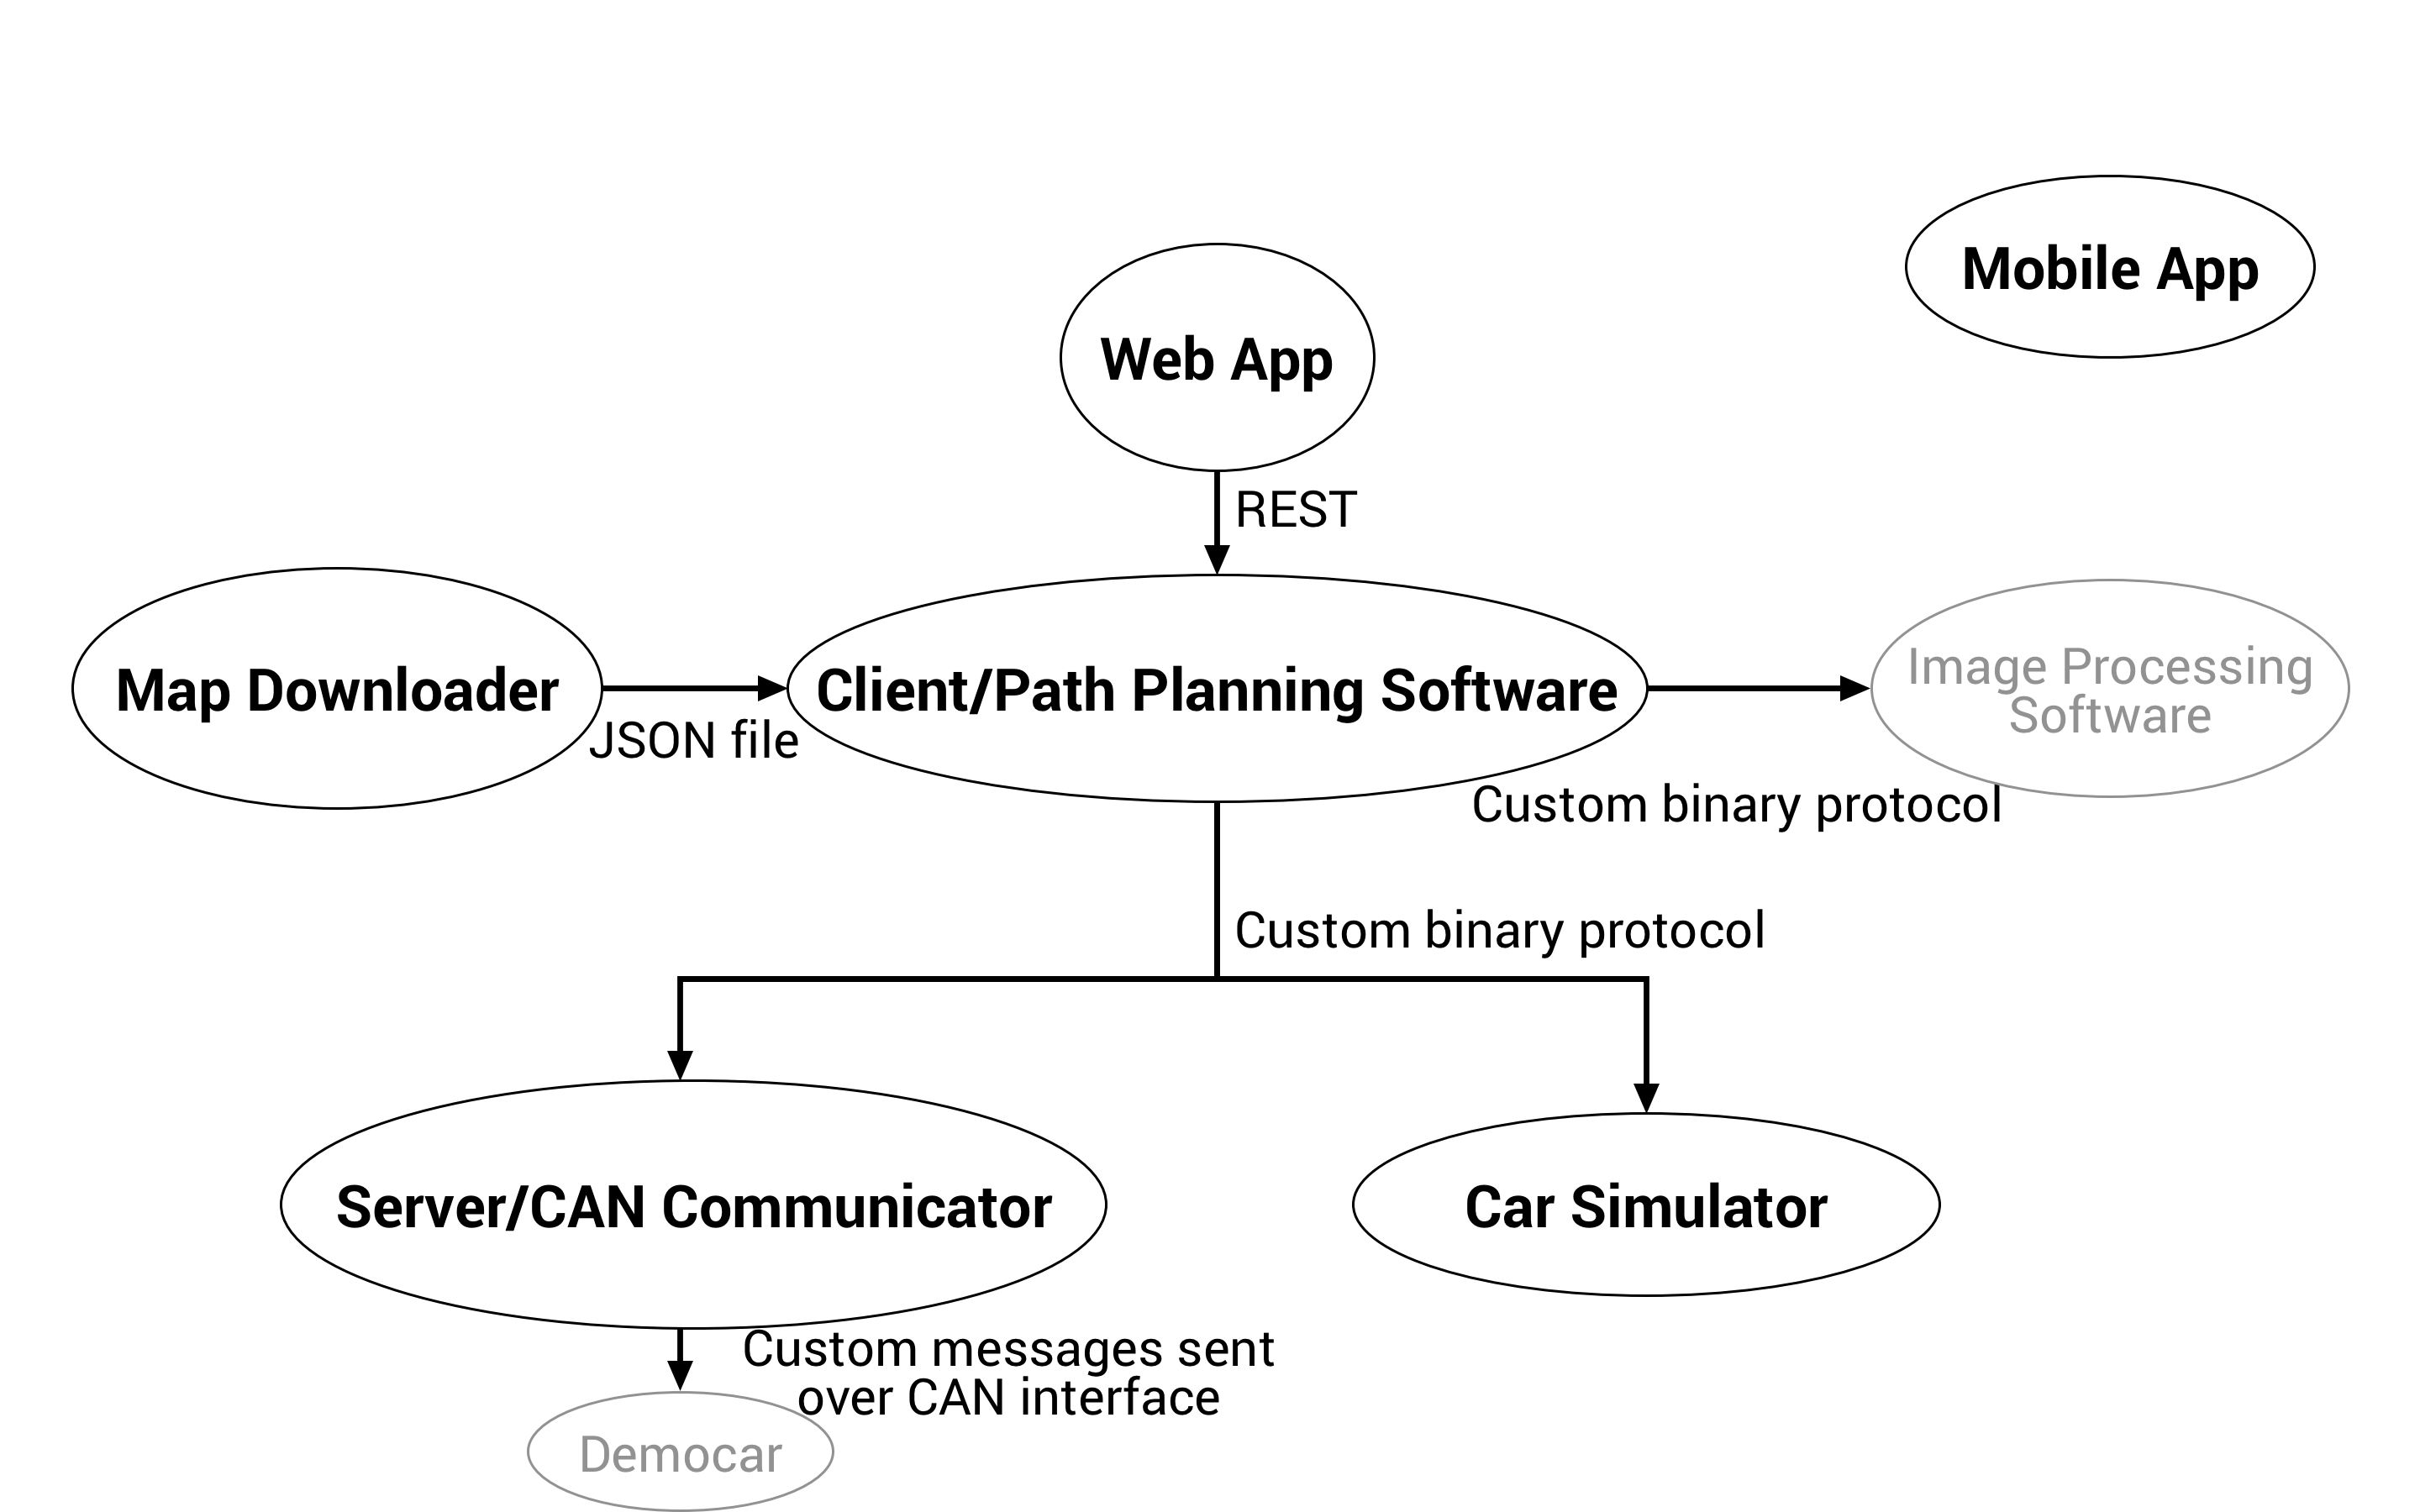
\includegraphics[width=0.9\columnwidth]{car-schema-full}
    \end{center}
\end{frame}

\section{Komponenty projektu}

\begin{frame}
    \frametitle{car-simulator}
\end{frame}

\begin{frame}
    \frametitle{car-can}
\end{frame}

\begin{frame}
    \frametitle{car-client}
\end{frame}

\begin{frame}
    \frametitle{car-webapp}
\end{frame}

\begin{frame}
    \frametitle{car-map-downloader}
\end{frame}

\begin{frame}
    \frametitle{GeoLogger}
\end{frame}

\section{Vývoj projektu a testování způsobů řízení}

\section{Zhodnocení projektu}

\end{document}

